\cotefile{69}
\scanpage{34}
\mspage{26}
% L1–4
Pour la \inserted{paire de} \deleted{bi}triangles
\figure{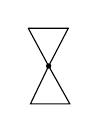
\begin{tikzpicture}[scale=.48]
\draw (-.54,1)--(.52,1)--(0,0)--(-.54,1) (0,0)--(-.48,-1)--(.56,-1)--cycle;
\fill (0,0) circle (2pt);
\end{tikzpicture}}
, \unsure{qu'il|qu'on|quitte} \unsure{faut|peut|à} noter que cette paire ``épinglée'' (pour en éliminer le groupe d'autom. du diagramme, qui est $\mathbb Z/4\mathbb Z$) équivaut :
% L5–8
la \unsure{b.trian|balise} épinglée (en éliminant le groupe d'autom $\mathfrak S_2$ de la \unsure{b.tri.|balise}). \deleted{équivaut : \unsure{la donnée|donc}} \inserted{\unsure{Du pt de vue non}} épinglé : sommet fixé \inserted{$u$}, avec un \unsure{un|ens.} des 2 triangles de sommet $u$, donc

% L9–11
a) un $Q_u$ de cardinal 5, décomposé en $Q'_u$ (de cardinal 2) et $Q''_u$ (de cardinal 3)

b) torseur sous $\Psi(Q_u,\mathbb F_2)=\operatorname{Ker}\bigl(\mathbb F_2^{Q'_u\amalg Q''_u}\longrightarrow\mathbb F_2\bigr)$

% L12–15. The two glosses stand directly underneath their factors.
\uline{Nb} de telles paires
\[
\underset{\substack{\text{sommet}\\u}}{\underline{27}}\cdot
\underset{\substack{\text{partie}\\\text{à 2 él.}\\\text{de }Q_u}}{\binom{5}{2}}
=270=2\cdot3^3\cdot5
\]

Groupe d'autom de $(C,\ \tikz[baseline=-.6ex,scale=.14]{\draw (-1,1.4)--(1,1.4)--(-1,-1.4)--(1,-1.4)--cycle;\fill(0,0) circle (3pt);})$.
\[
\simeq(\unsure{\mathfrak S|\mathfrak G}_2\times\mathfrak S_3)\cdot
\underset{\substack{\unsure{\shortparallel|\cup|\simeq}\\\mathbb F_2^4}}{\Psi(\mathbb F_2)}
\qquad\text{de cardinal }\begin{aligned} &2\cdot6\cdot16\\ &=2^6\cdot3\end{aligned}
\]
% The slant stroke at right links the two numerical lines.
\figure{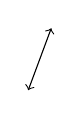
\begin{tikzpicture}[scale=.45]\draw[<->] (0,0)--(.65,1.75);\end{tikzpicture}}
% L16–17
On trouve bien comme produit
\[
2^7\cdot3^4\cdot5=\operatorname{card}W_{E_6}\qquad\ldots
\]
% archive sheet number: 33
\scanpage{35}
\mspage{27}
% L1–5
\textcircled{\scriptsize\unsure{13}} Cas du \uline{préprisme triangulaire} $D$
\figure{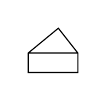
\begin{tikzpicture}[scale=.45]\draw (0,0)--(1.4,0)--(1.4,.55)--(.85,1.25)--(0,.55)--cycle (0,.55)--(1.4,.55);\end{tikzpicture}}
La donnée de ce diagramme dans $C$ équivaut : celle d'un carré
\figure{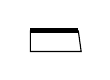
\begin{tikzpicture}[scale=.46]\draw (0,.58)--(0,0)--(1.4,0)--(1.32,.58);\draw[line width=2pt] (0,.58)--(1.32,.58);\end{tikzpicture}}
avec un côté marqué -- on l'étudiera plutôt avec le carré.

% L6–11
\textcircled{\scriptsize\unsure{14}} \unsure{Complexe|Complexes} cubique avec \uline{prisme triangulaire} \inserted{$D_6$} \inserted{ou : \uline{bitriangle} $D_7$}.
\figure{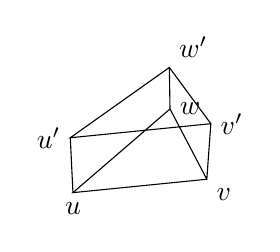
\begin{tikzpicture}[scale=.85]
\coordinate (u) at (0,0); \coordinate (v) at (2,.2); \coordinate (w) at (1.45,1.25);
\coordinate (U) at (-.04,.82); \coordinate (V) at (2.06,1.03); \coordinate (W) at (1.44,1.87);
\draw (u)--(v)--(w)--cycle (U)--(V)--(W)--cycle (u)--(U) (v)--(V) (w)--(W);
\node[below] at (u) {$u$};\node[below right] at (v) {$v$};\node[right] at (w) {$w$};
\node[left] at (U) {$u'$};\node[right] at (V) {$v'$};\node[above right] at (W) {$w'$};
\end{tikzpicture}}
Il donne naissance, en \unsure{fermant|formant} les triangles sur les arêtes latérales, à un bitriangle à paire de triangles \inserted{disjoints} distinguée $\{\{u,v,w\},\{u',v',w'\}\}$ (épinglage partiel).
\figure{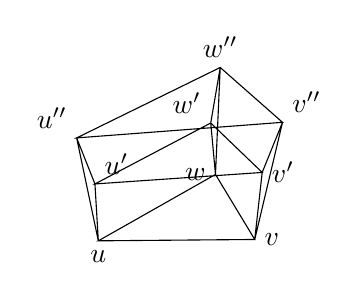
\begin{tikzpicture}[scale=.86]
\coordinate(u) at (.32,0);\coordinate(v) at (2.63,.02);\coordinate(w) at (2.05,.98);
\coordinate(U) at (.27,.84);\coordinate(V) at (2.74,1.01);\coordinate(W) at (1.98,1.74);
\coordinate(A) at (0,1.52);\coordinate(B) at (3.04,1.75);\coordinate(C) at (2.12,2.56);
\draw (u)--(v)--(w)--cycle (U)--(V)--(W)--cycle (A)--(B)--(C)--cycle (u)--(U)--(A)--cycle (v)--(V)--(B)--cycle (w)--(W)--(C)--cycle;
\node[below] at(u){$u$};\node[right] at(v){$v$};\node[left] at(w){$w$};\node[above right] at(U){$u'$};\node[right] at(V){$v'$};\node[above left] at(W){$w'$};
\node[above left] at(A){$u''$};\node[above right] at(B){$v''$};\node[above] at(C){$w''$};
\end{tikzpicture}}

% L12–22
Étudions d'abord les bitriangles, au nb de 120 (cf p. 10) ; \deleted{le gpe des autom d'un diagramme $\Delta$ $(\simeq D_7)$, est \unsure{$\mathfrak S_2$|$\mathfrak G_2$}.} La donnée d'un diagramme de type $D_7$ équivaut : celle d'un ens $\inserted{\Delta_0}$ de cardinal 9, muni de \inserted{un ens $\{\pi,\pi'\}$ de} deux partitions de type $(3,3,3)$, de telle façon que l'application $\Delta_0\unsure{-|\longrightarrow}(\Delta_0/\pi\times\Delta_0/\pi')$ soit bijective, ou encore d'un ens $\inserted{T}$ de cardinal 6 (l'ens des 6 triangles de $\Delta$) et d'une partition de $T$ de type $(3,3)$, i.e. d'une application $T\longrightarrow I$ de degré 3, \deleted{\unsure{cardinal}} $\operatorname{card} I=2$. (\unsure{bon|car}. alors $\Delta_0=\prod_{i\in I}T_i\quad\ldots$) Le gpe des autom
% archive sheet number: 34
\scanpage{36}
\mspage{28}
% L1–6
de $\Delta$ \deleted{est} s'identifie au gpe des autom de $(T\longrightarrow I)$, une fois choisi un iso. entre les deux fibres de $T\to I$, il s'identifie au produit $\tfrac12$ direct
\[
\underset{\substack{\shortparallel\\\mathfrak S_2}}{\unsure{\mathfrak S|\mathfrak G}_{\unsure{I|2}}}\cdot\prod_{i\in I}\mathfrak S_{T_i}
\]
de cardinal 72 (\uline{égal} au nb de racines\ldots).

% L7–15
Si on a un plongt $\Delta_0\xrightarrow{i} C$, \deleted{les} \inserted{le gpe des} autom de $(C,i(\Delta_0)=\Delta)$ s'applique sur celui de $\Delta$, le noyau étant d'ordre 6, isomorphe : $\mathfrak S_3$. On va associer à $i(\Delta)$ un ens $V^*$, \unsure{très strict|trois élémts|triple}, qui sera canoniqut isom, pour tt $u\in i(\Delta)$, à \deleted{\unsure{un}} l'ens \inserted{$V^*(u)$} des trois triangles de $C$ de sommet $u$, distinct des 2 triangles $\in\Delta$. Il faut donc établir

% L16–20; left rule along the four lines of the lemma.
\uline{Lemme} \unsure{1}\quad $\exists!$ syst. transitif d'iso. entre les $V^*(u)$ $(u\in\Delta)$ tels que si $x\in C-\Delta$, et si $x$ est lié à $u,v\in\Delta$, alors les triangles $\operatorname{tr}(u,x)\in V^*(u)$ et $\operatorname{tr}(v,x)\in V^{\unsure{1|*}}(v)$ se correspondent

% L21–25
Utiliser l'épinglage des p. 8 et 9

On trouve que
\[
\operatorname{Aut}(C,\Delta)\longrightarrow
\underset{\substack{\shortparallel\\\mathfrak S_2\cdot(\mathfrak S_3\times\mathfrak S_3)}}{\operatorname{Aut}(\Delta)}
\times\underset{\substack{\shortparallel\\\mathfrak S_3}}{\operatorname{Aut}(\unsure{W|V}^*)}
\]
est un iso. Il faut donc expliciter comment on reconstitue $(C,\Delta)$
% archive sheet number: 35
\scanpage{37}
\mspage{29}
% L1–2
via le diagramme $\Delta$ et l'ens $V^*$ de cardinal 3.

% L3–7
\uline{Lemme 2} \quad a) $\forall x\in C-\Delta$, soit $\Delta(x)=\Delta\cap E(x)_0$. Alors $[\operatorname{card}\Delta(x)=3,\ \text{et}]$ les deux applications $\prod_{j\in I}T_j\simeq\Delta\hookrightarrow\!\longrightarrow T_i$ $(i\in I)$ définissent des bijections $\Delta(x)\simeq T_i$ i.e. $\Delta_x$ est le graphe d'une bijection $T_i\simeq T_{i'}$ (si \deleted{\unsure{$i,i'$|$i\ne i'$}}, $I=\{i,i'\}$).
% L8–14
b) Soit \deleted{\unsure{l'ens}} $\deleted{\unsure{E}}\unsure{F'|T'|\mathbb F'}$ l'ens des parties \inserted{$\Delta'$} de $\Delta$ \deleted{\unsure{$(x)$}} ayant les propriétés précédentes [i.e. de cardinal 3, et formé de p$^{\rm ts}$ 2 à deux non liés \inserted{ds $\Delta$}], et \unsure{considérer|considérons} les applications canoniques $(C-\Delta)\longrightarrow F$ et $(C-\Delta)\longrightarrow V^*$, d'où $(C-\Delta)\longrightarrow F'\times V^*$. Cette application est bijective.

% L15–22
Il faut expliciter la relation de \deleted{\unsure{incidence}} \inserted{liaison} dans $C\simeq\Delta\amalg(F'\times V^*)$. On a déjà la relation de liaison pour deux él \deleted{\unsure{qui}} \inserted{$x,y$ si $x,y$} sont dans $\Delta$, ou si $x\in\Delta$, $y\unsure{\in|=}(\Delta(y),v(y))\in F'\times V^*$ [c'est la relation $x\in\Delta(y)$]. Il reste à l'expliciter si $x,y\in F'\times V^{\unsure{\wedge|*}}$, $x=(\Delta(\deleted{\unsure{y}}x),v(x))$, $y=(\Delta(y),v(y))$. On trouve que $x,y$ \inserted{distincts} sont liés ssi
\[
\left\{\begin{aligned}
&\text{ou bien }\Delta(x)\cap\Delta(y)\ne\varnothing,\quad v(x)=v(y)
&&(\text{donc }\operatorname{card}\Delta(x)\cap\Delta(y)=1)\\
&\text{ou bien }\Delta(x)\cap\Delta(y)=\varnothing,\quad v(x)\ne v(y)
\end{aligned}\right.
\]
% archive sheet number: 36
\scanpage{38}
\mspage{30}
% L1–5
Justification a priori de cette description, on considère le graphe ainsi construit à l'aide de $\Delta,V^*$ ; on vérifie qu'il satisfait aux propriétés caractéristiques d'un complexe cubique (th. p. 1)\ldots

\medskip\centerline{\rule{1.2cm}{.3pt}}\medskip
% L6–13
Bases orthogonales à un bitriangle $\Delta$.
Ce sont aussi les bases $b\subset C-\Delta$ (cf p. \unsure{29|24} bis), donc les systèmes de 6 \unsure{élémt|éléments} mutuellmt non liés de $\unsure{F'|T'|\mathbb F'}\times V^*$. Considérons le \unsure{tor.|rev.|tors.} \inserted{$\widetilde I$} d'ordre 2 de $I$ des permutations circulaires sur les fibres de $T\to I$, et considérons $J=\underset{\substack{(\text{produit}\\\text{de Baer}\\i\in I)}}{\bigwedge^{\unsure{\prime}}}\widetilde I_i$, qui est un ens à 2 él. L'ens des bases cherchées est en corr. 1--1 avec $\operatorname{Mon}(J,V^*)$.
% L14–23
Si on a une injection $J\overset{\varphi}{\hookrightarrow}V^*$, on lui associe l'ens \inserted{$b_\varphi$} des $\{x=(\Delta(x),v(x))\in F'\times V^*$ tels que $\varphi(\deleted{\unsure{\Delta}}\text{image de }\Delta(x)\text{ dans }J)=v(x)$ ; ils sont évidemt de cardinal 6 $[\inserted{\text{car }}b_\varphi\xrightarrow{\sim}F')$ \deleted{\unsure{est}}, et ses éléments sont mutuellmt non liés car $v(x)=v(y)$ implique que $\Delta(x)$ et $\Delta(y)$, en \unsure{tant} que $T_i\xrightarrow{\sim}T_j$ $(I=\{i,j\})$, diffèrent par un él. du gpe \uline{alterné} $A_3$, donc $\Delta(x)\cap\Delta(y)=\varnothing$, ce qui implique $x,y$ non liés.
% archive sheet number: 37
\scanpage{39}
\mspage{31}
% L1–6
Donc la cat. des triplets $(C,\Delta,b)$ d'un complexe cubique $C$, muni d'un bitriangle $\Delta$ et d'une base $b$ orthogonale à \unsure{celle-ci|celui-ci}, \uline{équivaut} à celle des $\Delta$ (car $V^*$ se réconstitue comme
\[
V^*\simeq J\amalg\{\mathrm{pt}\}
\]
% L7–9
Donc le groupe des autom. d'une telle structure est $\simeq\operatorname{Aut}(\Delta)\simeq\unsure{\mathfrak S|\mathfrak G}_2\cdot(\mathfrak S_3\times\mathfrak S_3)$ de card. 72.

% L10–19
Pour $C$ fixé, l'ens des couples $(\Delta,b)$ est de cardinal $\inserted{120\cdot6=}720$, donc pour $b\inserted{=\unsure{T'|F'|\mathbb F'}}$ fixé, l'ens des $\Delta$ correspondants est de cardinal $10=\binom63\frac12={}$\inserted{cardinal de l'}ens des partitions \inserted{$\{T'_1,T'_2\}$} de $T'$ en deux parties à 3 éléments. Or, pour une telle partition, on déduit un bitriangle orthogonal à $b$, en prenant \inserted{l'ens} des $(\{ij\})_{\substack{i\in T'_1\\j\in T'_2}}$, correspondant à l'ens \inserted{$T$} des 6 triangles \inserted{$t_{\sigma}={}$}$(\{i,\sigma i\})_{i\in T'_1}$, où $\sigma\in\operatorname{Isom}(T'_1,T'_2)$.
% L20–23. Two pen strokes in the left margin beside this passage.
\deleted{Ainsi,} En $=$ temps, on tombe sur une \uline{autodualité} dans la catégorie des ens de cardinal 6 munis d'une partition de type $(3,3)$ \ldots
% archive sheet number: 38
\scanpage{40}
\mspage{32}
% L1–5
Considérons les 6 \deleted{\unsure{racines|racines, et}} \inserted{bases} orth. à un bitriangle $(u,v,w,\ u'=\alpha_4,v'=\beta_4,w'=\gamma_4,u''=\alpha'_{\unsure{4|2|1}},v''=\beta'_4,w''=\gamma'_4)$ \deleted{\unsure{dans le}} avec les notations des pp. 9, 10. On trouve les bases \deleted{de la forme}
% L6–11
\[
b=(\alpha_1,\alpha'_2,\beta_1,\beta'_2,\gamma_1,\gamma'_2)
\]
et celles qui s'en déduisent par les \inserted{6} permutations de $\{1,2,3\}$. La base duale à la base écrite est $b'=(\alpha_2,\alpha'_1,\beta_{\unsure{2|3}},\beta'_1,\gamma_2,\gamma'_1)$, la racine correspondante à $b$ est
\[
\alpha_2-\alpha_1=\alpha'_1-\alpha'_2=\beta_2-\beta_1=\beta'_1-\beta'_2=\gamma_2-\gamma_1=\gamma'_1-\gamma'_2,
\]
% L12–15
on trouve donc les 6 racines de la forme $\alpha_i-\alpha_j$ $(i\ne j,\ 1\le i,j\le3)$. Elles forment évidemment un \uline{syst. de racines de type $A_2$}

\figure{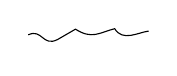
\begin{tikzpicture}[scale=.6]\draw (0,0)..controls (.3,.14) and (.3,-.26)..(.62,-.10)--(1,.12)..controls (1.35,-.1) and (1.49,.04)..(1.83,.13)..controls (2,-.15) and (2.32,.05)..(2.55,.08);\end{tikzpicture}}
% L16–19
expliciter a) les positions relatives d'un bitriangle \inserted{$\Delta$} et d'un triangle $t$. Il y en a trois
\[
\left\{\begin{aligned}
&t\subset\Delta\quad\text{i.e. }\operatorname{card}t\cap\Delta=3\\
&\operatorname{card}(t\cap\Delta)=1\\
&\deleted{\unsure{t\in}}t\cap\Delta=\varnothing\quad\text{i.e. }\operatorname{card}(t\cap\Delta)=0
\end{aligned}\right.
\quad\begin{array}{|r}6\\3\cdot9\\12\\\hline\hline45\end{array}
\]
% L20–25
b) Les positions relatives d'une base (ou bibase) et d'un bitriangle (il semble qu'il y en ait trois : $b$ orthogonale à $\Delta$, $b$ \inserted{non orth. à $\Delta$ mais} orthogonale à au moins un triangle de $\Delta$ (Alors il est \unsure{orth.} à \unsure{exactt|exactement} 2 triangles \unsure{dont|et dont} la réunion est de cardinal 5 \ldots), enfin $b$ orth. à aucun triangle de $\Delta$\ldots
% margin note written sideways
\margin{c) positions relatives de deux bitriangles ???}
% archive sheet number: 39
\scanpage{42}
\mspage{1}
% L1–7
Les 27 droites de la surface cubique, et le syst. de racines $E_6$.

I. \quad $P$ plan projectif (sur corps $k$ alg. clos p. ex.)

$S=\{s_1,\ldots,s_6\}$ ens de 6 pts de $P$ \deleted{\unsure{dont} trois ne sont pas} \inserted{\unsure{non|pas}} alignés \inserted{trois à trois} \inserted{et pas \inserted{tous} sur une même conique}

$\widetilde P$ déduit de $P$ en faisant éclater $S$

$\widetilde S=\sum_1^6D_i$ image inverse de $S$

$D_{ij}$ $(1\le i\ne j\le6)$ image inv. propre de la droite qui joint $s_i,s_j$

$D'_i$ image inverse propre de \uline{la} conique de $P$ passant par $S-\{s_i\}$
\margin{\uline{vérifier}}

% L8–14
On a
\margin{\uline{vérifier} cf calculs plus bas}
\[
\left\{\begin{aligned}
D_i\cap D_j&=\varnothing &&\text{si }i\ne j\\
D_i\cap D_{j\unsure{k|h}}&\ne\varnothing &&\text{sss }i\in\{j,h\}\\
D'_i\cap D'_j&=\varnothing &&\text{si }i\ne j\\
D'_i\cap D_{jh}&\ne\varnothing &&\text{sss }i\in\{j,h\}\\
D_i\cdot D'_j&\ne\varnothing &&\text{sss }i\ne j\\
D_{ij}D_{k\ell}&\ne\varnothing &&\text{sss }\{i,j\}\cap\{k,\ell\}\text{ de card. }0\text{ ou }2
\end{aligned}\right.\tag*{(\unsure{0|$\ast$})}
\]
% L15–22
On calcule dans $E=A^1(\widetilde P)=\operatorname{Pic}(\widetilde P)$, on désigne par
\[
\eta,\ (\unsure{\zeta|\xi}_i)_{1\le i\le6}\tag*{(1)}
\]
l'image inverse de $\operatorname{cl}(O_P(1))$ et les classes des $D_i$, par $\zeta'_i$ les classes des $D'_i$, par $\zeta_{ij}$ celles des $D_{ij}$. On trouve
\[
\zeta_{ij}=\eta-\zeta_i-\zeta_j\tag*{(2)}
\]
\[
\zeta'_i=2\eta-\sum_{\alpha\ne i}\zeta_i=2\eta-\zeta+\zeta_i\tag*{(3)}
\]
i.e.
\[
\zeta'_i-\zeta_i=2\eta-\zeta\tag*{(3 bis)}
\]
en posant
\[
\zeta=\sum_1^6\zeta_\alpha\tag*{(4)}
\]
Posons aussi
\[
\zeta'=\sum_1^6\zeta'_\alpha=12\eta-5\zeta\tag*{(4')}
\]
et définissons $\eta'$ par
\[
2\eta-\zeta=-(2\eta'-\zeta')\qquad\text{i.e. }\ 2(\eta+\eta')=\zeta+\zeta'\tag*{(5)}
\]
i.e (compte tenu de (3 bis)) :
\[
\zeta_i-\zeta'_i=2\eta'-\zeta'\tag*{(5 bis)}
\]
On trouve, posant
\[
\lambda=3\eta-\zeta\tag*{(6)}
\]
% archive sheet number: 41
\scanpage{43}
\mspage{2}
% L1–6
les formules
\[
\unsure{\zeta|\xi}+\zeta'=12\eta-4\zeta=\deleted{\unsure{6}}4\lambda\tag*{(7)}
\]
donc (5) s'écrit \deleted{$\eta+\eta'=2\lambda$} \inserted{(en divisant par 2)}
\[
\eta+\eta'=2\lambda\tag*{(8)}
\]
ou encore
\[
\eta'=5\eta-2\zeta\tag*{(\unsure{8|9} bis)}
\]
% L7–13
Notons que $\lambda$ provient de l'application rationnelle $P\longrightarrow\mathbb P^3$ définie par le système des cubiques qui passent par $S$, laquelle devient régulière sur $\widetilde P$ et définit une immersion $\widetilde P\hookrightarrow\mathbb P^3$ dont l'image est une surface cubique. (En particulier, $\lambda$ est ample\ldots) \deleted{On}

% slanted
\margin{$\unsure{K|\lambda}=-3\unsure{\lambda|\eta}$ ($K$ classe canonique) ce qui caractérise $\lambda$ de façon intrinsèque, à la surface $\widetilde P$ $=X$. Du $=$ coup, l'inclusion $X\hookrightarrow\mathbb P^3$ (var. de \unsure{Sév.} Brauer) est intrinsèque à $X$, ainsi que les $D_i,D'_i,D_{ij}$, qui sont les seules droites de $\mathbb P^3$ contenues dans $X$ -- a fortiori, les 27 élts $\zeta_i,\zeta'_i,\zeta_{ij}\in E$ sont intrinsèques à $X$.}

Calculons la forme intersection sur $\widetilde P$.

On a
\[
\eta^2=1,\qquad \zeta_i^2=-1\qquad \eta\cdot\zeta_i=0,\quad\zeta_i\zeta_j=0\quad\text{si }i\ne j\tag*{(10)}
\]
d'où facilement
\[
\eta'{}^2=1,\quad\zeta'_i{}^2=-1,\quad\eta'\cdot\zeta'_i=0,\quad\zeta'_i\zeta'_j=0\quad\text{si }i\ne j.\tag*{(11)}
\]
\unsure{Et|et|On a} aussi
\[
\lambda^2=3\qquad(=\lambda\eta=\lambda\eta')\tag*{(12)}
\]
\[
\lambda\zeta_i=\lambda\zeta'_i=\lambda\zeta_{ij}=1\tag*{(13)}
\]
% L19–23
La relation (12) signifie que l'immersion $\widetilde P\longrightarrow\mathbb P^3$ a comme image une surface cubique, la relation (13) que les images dans $\mathbb P^3$ des 27 \inserted{$=6+6+15$} courbes $D_i,D'_i,D_{ij}$ sont des \uline{droites}.

Notons encore
\[
\zeta_i\zeta'_j=\begin{cases}0&\text{si }i=j\\1&\text{si }i\ne j\end{cases}\tag*{(14)}
\]
\unsure{(}
% archive sheet number: 42
\scanpage{44}
\mspage{3}
% L1–4
\[
\unsure{\zeta|\xi}_i\zeta_{jh}=\zeta'_i\zeta_{jh}=
\begin{cases}0&\text{si }i\notin\{j,h\}\\1&\text{si }i\in\{j,h\}\end{cases}\tag*{(15)}
\]
\[
\zeta_{ij}\zeta_{h\ell}=\begin{cases}
0&\text{si }\operatorname{card}\{i,j\}\cap\{h,\ell\}=1\\
1&\text{si }\{i,j\}\cap\{h,\ell\}=\varnothing
\end{cases}\tag*{(16)}
\]
% L5–13
ce qui précise (0) : les \inserted{27} droites, quand \deleted{elles} \inserted{deux} se rencontrent, se rencontrent en \unsure{exactt|exactement} un pt avec int. transversale (\unsure{ou a priori|on espère} !) On vérifie de plus que tte droite parmi les 27 en rencontre exactement 10 autres ; p. ex. $D_i$ rencontre les $D'_j$ \deleted{\unsure{$j\ne i$}} \inserted{et} $D_{ij}$ $(j\ne i)$ $D'_i$ les $D_j$ et $D_{ij}$ $(j\ne i)$, $D_{12}$ rencontre $D_1,D_2,D'_1,D'_2\ ;\ D_{3,4}\ D_{5,6}\ D_{3,5}\ D_{4,6},D_{3,6},D_{4,5}$ \ldots On vérifie aussi que si $\delta,\delta'$ parmi \deleted{les} \inserted{l'ens $\Delta$ des} 27 droites se rencontrent, $\exists!\,\delta''\in\Delta$ \deleted{parmi} \unsure{dt|tel} que $\delta''$ rencontre $\delta$ et $\delta'$\ldots

% L14–22
II) Soit, sur un anneau $k$ \inserted{$\ne0$} (p. ex. $k=\mathbb Z$) ; un module \deleted{engendré par} \inserted{avec} des éléments $\overbrace{\eta,\zeta_i,\eta',\zeta'_i\qquad(1\le i\le6)}$ satisfaisant (posant \deleted{$\zeta=\sum\zeta_i,\zeta'=\sum\zeta'_i$})
\[
\zeta=\sum_1^6\zeta_i,\qquad\zeta'=\sum_1^6\zeta'_i\tag*{\textcircled{a} (déf)}
\]
\[
2(\eta+\eta')=\zeta+\zeta'\qquad\text{i.e.}\qquad2\eta-\zeta=-(2\eta'-\zeta')\tag*{\textcircled{b}}
\]
et de plus
\[
\zeta'_i-\zeta_i=2\eta-\zeta\qquad\text{i.e.}\qquad\zeta_i-\zeta'_i=2\eta'-\zeta'\tag*{\textcircled{c}}
\]
Alors on a les relations
\[
\left\{\begin{aligned}
\zeta'_i&=2\eta-\zeta+\zeta_i=2\eta-\sum_{\alpha\ne i}\zeta_i\\
&\deleted{\unsure{\eta'=5\eta-2\zeta}}\\
\zeta'&=12\eta-5\zeta
\end{aligned}\right.\tag*{(d)}
\]
\deleted{donc $\zeta+\zeta'=4\lambda=4\lambda'$ \unsure{avec} $\left\{\begin{aligned}\lambda&=3\eta-\zeta\\\lambda'&=3\eta'-\zeta'\end{aligned}\right.$} \unsure{alors}
% archive sheet number: 43
\scanpage{45}
\mspage{4}
% L1–6
et les relations symétriques
\[
\left\{\begin{aligned}
\unsure{\zeta|\xi}_i&=2\eta'-\zeta'+\zeta'_i=2\eta'-\sum_{\alpha\ne i}\zeta'_i\\
&\deleted{\unsure{\eta=5\eta'-2\zeta'|\eta=5\eta'-2\eta'}}\\
\zeta&=12\eta'-5\zeta'
\end{aligned}\right.\tag*{(d')}
\]
d'où
\[
\zeta+\zeta'=4\lambda=4\lambda'\quad\text{avec}\quad
\lambda=3\eta-\zeta,\ \lambda'=3\eta'-\zeta'\tag*{(e)}
\]
\deleted{Donc}, On aura \deleted{\unsure{par} $4\unsure{(\lambda|(\mathrm e)}$} $4\lambda=4\lambda'$ i.e. $4(\lambda'-\lambda)=0$, mais on suppose qu'on a $=$
\[
3\eta-\zeta=3\eta'-\zeta'\overset{\mathrm{dfn}}=\lambda\tag*{\textcircled{f}}
\]
\margin{\uline{NB} conséquence de ce qui précède si 2 inv. dans $k$ (ou ds $M$)}
% L7–12
et on trouve \inserted{$3\eta'=3\eta-\zeta+\zeta'=15\eta-6\zeta$ compte tenu de \textcircled{b} donnant $2\eta'\deleted{\unsure{+\zeta}}=\zeta+\zeta'-2\eta=10\eta-4\zeta$}
\[
\left\{\begin{aligned}\eta+\eta'&=2\lambda\\\zeta+\zeta'&=4\lambda\end{aligned}\right.\tag*{(f)}
\]
\[
\left\{\begin{aligned}\eta'&=5\eta-2\zeta\\\eta&=5\eta'-2\zeta'\end{aligned}\right.\tag*{(g,g')}
\]
On voit que pour que $(\eta,(\zeta_i))$ soit une famille gén. (basique) \unsure{de|dans} $M$, il f et s qu'il en soit de $=$ de $(\eta',(\zeta'_i))$. \deleted{\unsure{Posant|Posons}} \inserted{On a}
\[
\eta-\zeta_i-\zeta_j=\eta'-\zeta'_i-\zeta'_j\quad(\overset{\mathrm{dfn}}=\zeta_{ij})\tag*{(\deleted{\unsure{f}}h)}
\]
% L13–20
Le module engendré par \deleted{\unsure{l'ens des}} $(\eta,(\zeta_i))$ ou par $(\eta',(\zeta'_i))$, ou par la \deleted{\unsure{2}} famille de 27 él. $(\zeta_i)$ $(\zeta'_i)$ $(\zeta_{ij})$ [ou \unsure{seult|même} $((\zeta_i),\zeta_{12})$ disons] sont les $=\text{s}$\ldots

Supposons qu'on \deleted{existe} \inserted{donne} sur $M$ une forme bil. \inserted{sym.}, notée $x\cdot y$. \deleted{telle que} \inserted{Alors} les relations
\[
\eta^2=1,\quad\zeta_i^2=-1,\quad\eta\zeta_i=0,\quad\zeta_i\zeta_j=0\quad\text{si }i\ne j\tag*{(i)}
\]
sont équiv. aux relations sym.
\[
\eta'{}^2=1,\ \zeta'_i{}^2=-1,\quad\eta'\zeta'_i=0,\quad\zeta'_i\zeta'_j=0\quad\text{si }i\ne j\tag*{(\deleted{\unsure{g}}i')}
\]
et elles impliquent que $(\eta,(\zeta_i))$ font une famille libre (ou $(\eta',(\zeta'_i))$ aussi) -- donc
% archive sheet number: 44
\scanpage{46}
\mspage{5}
% L1–6
une base s'ils sont générateurs. Inversement, si ils font une base, $\exists!$ forme bil. sym. satisfaisant les conditions équivalentes (i), (i'). On aura alors les formules (12) à (16) de (I). On suppose dorénavant qu'on est dans cette situation.

% L7–13
\unsure{§} Considérons les \unsure{27|17} éléments $\unsure{\zeta|\xi}_i,\zeta'_i$ \inserted{$(1\le i\le6)$}, $\zeta_{ij}$ $(1\le i\ne j\le6)$, qui dans la base $(\eta,(\zeta_i))$ s'écrivent
\[
\begin{aligned}
\zeta_i&=\zeta_i\\
\zeta'_i&=2\eta-\sum_{\alpha\ne j}\zeta_i\\
\zeta_{ij}&=\eta-\zeta_i-\zeta_j\quad\inserted{(i\ne j)}
\end{aligned}
\]
\margin{\uline{NB} \deleted{les} $\delta$ engendrent $\widehat E$ (il suffit $=$ des $\zeta_i$ et d'\uline{un} $\zeta_{ij}$)}
donc sont tous distincts. \inserted{Soit \deleted{\unsure{$\Delta$ leur}} $\Delta_{\unsure{0|X}}$ leur ens.} On met dessus une structure de graphe en notant \deleted{\unsure{convenant}} que si $\delta,\delta'\in\Delta_{\unsure{x|k|X}}$, \inserted{$\delta\ne\delta'$}, on a $\delta\cdot\delta'=0$ ou 1, \inserted{(NB $\delta^2=\delta'{}^2=-1$)} et \unsure{en considérant|on considère} \deleted{$\delta,\delta'$ liés sss \unsure{à|$\delta$}}
\[
\delta,\delta'\ \inserted{\in\Delta_x,\ \delta\ne\delta'}\ \text{liés ssi}\qquad\delta\delta'=1\qquad\text{i.e. }\delta\delta'\ne0.\tag*{(j)}
\]
% L14–21
Donc $\zeta_i$ est lié aux él. $\zeta'_j$ $(j\ne i)$ et $\zeta_{ij}$ $(j\ne i)$ \unsure{exclt|exactement} (soit 10 él.), $\zeta'_i$ est lié aux él. $\zeta_j$ $(j\ne i)$ et $\zeta_{ij}$ $(j\ne i)$ \unsure{exclt|exactement} (soit encore 10 éléments) et $\zeta_{ij}$ \inserted{$(i\ne j)$} est lié à $\zeta_i,\zeta_j,$ \inserted{$\zeta'_i,\zeta'_j,$} et à $\zeta_{k\ell}$ $(k\ne i,j,\ell\ne i,j,k\ne\ell)$ en nombre $\binom42=6$, donc en tout encore 10 éléments. \deleted{Enfin,} Les \deleted{couples} \inserted{paires} de sommets liés sont donc
% archive sheet number: 45
\scanpage{47}
\mspage{6}
% L1–2
exactement les $\{\unsure{\zeta|\xi}_i,\zeta'_j\}$ $(i\ne j)$ $\{\zeta_i,\zeta_{ij}\}$ $(i\ne j)$ $\{\zeta'_i,\zeta_{ij}\}$ $(i\ne\unsure{j})$ et $\{\zeta_{ij},\zeta_{k\ell}\}$ \inserted{avec $\{i,j\}\cap\{k,\ell\}=\varnothing$}. \deleted{On note que}

% L3–8
\uline{Lemme} Si $\delta,\delta'$ sont deux sommets (distincts) liés alors $\exists!\,\delta''$ lié à $\delta$ et $\delta'$.

En effet, pour $\{\zeta_i,\zeta'_j\}$ c'est $\zeta_{ij}$, pour $\{\zeta_i,\zeta_{ij}\}$ c'est $\zeta'_j$, pour $\{\zeta'_i,\zeta_{ij}\}$ c'est $\zeta_j$ ; pour $\{\zeta_{ij},\zeta_{k\ell}\}$ c'est $\zeta_{rs}$ où $r,s$ sont les deux entiers $1\le\ \le6$ distincts de $i,j,k,\ell$.
% slanted; clipped at right edge
\margin{\unsure{NB} \illegible{1}}

% L9–14
\uline{Définition} Graphe cubique = graphe isomorphe au graphe \unsure{standart|standard} précédent (construit en prenant \deleted{\unsure{$I$}} $[1,6]\amalg[1,6]\amalg\unsure{\mathfrak P_2|\mathscr P_2}([1,6])$ comme ens de sommets).

À un tel graphe \inserted{$\Delta$ (\unsure{comme : tt graphe|comme à tout graphe|comme : tel graphe})} on associe (pour un anneau comm. $k$ donné) la forme bilinéaire \inserted{sym.} sur $k^{[\Delta]}\times k^{(\Delta)}$ donnée par
\[
\delta\delta'=\begin{cases}
-1&\text{si }\delta=\delta'\\
1&\text{si }\delta\ne\delta',\ \delta\text{ et }\delta'\text{ liés}\\
0&\text{si }\delta\unsure{\ne|=}\delta',\ \delta\text{ et }\delta'\text{ non liés}
\end{cases}
\]
% L15–22
Considérons le noyau \inserted{$N(\Delta)$} de cette forme, et soit $\widehat E_k(\Delta)=k_{\unsure{\zeta|?}}^{[\Delta]}/N(\Delta)$, qui est donc muni d'une forme bilinéaire sym. (non dégénérée au sens faible)

Dans le cas d'un graphe cubique, celle-ci est donc non dégénérée (et $\widehat E_k(\Delta)$ est un module libre de rang 7) comme on voit sur le cas standard.
% archive sheet number: 46
\scanpage{48}
\mspage{7}
% L1–5
Base ordonnée $(\alpha_{\unsure{i}})_{1\le i\le6}$ d'un graphe cubique : déduite de $(\unsure{\zeta|\xi}_i)_{1\le i\le6}$ dans $\Delta_0$ standard par \deleted{\unsure{la}} un isom. Base $(\alpha_i)_{i\in\underline I}$ : $\operatorname{Card}\underline I=6$, et on peut y ordonner \inserted{$\underline I,\ \underline I\simeq[1,6]$} de façon que la famille devienne une base ordonnée. Partie basique de $S$.

% L6–14
\uline{Prop} (\unsure{trivial|triviale}) $u\mapsto u((\zeta_i))$ définit une \deleted{isom} bijection de $\operatorname{Isom}(\Delta_0,\Delta)$ avec l'ens des bases ordonnées de $\Delta$ (qui est donc un torseur à droite sous $W_0=\operatorname{Aut}(\Delta_0)$, à gauche sous $W=\operatorname{Aut}(S)$). Considérons l'inclusion évidente $\unsure{\mathfrak S|\mathfrak G}_6\subset W_0$. Alors $u\mapsto u(\{\zeta_i\}_{i\in\underline I}$ définit par passage au quotient une bijection
\[
\operatorname{Isom}(\Delta_0,\Delta)/\mathfrak S_6\simeq
\begin{aligned}&\text{ens des parties}\\&\text{basiques de }\Delta.\end{aligned}
\]
% L15–24
\uline{Dém} Pour le premier pt, il suffit de voir que tt autom $u$ de $S$ tel que $u(\zeta_i)=\zeta_i$ \inserted{$\forall i$} est l'identité. Or comme $\zeta'_i$ est l'unique élément de $\Delta$ \deleted{distinct de $\zeta_i$ et des autres $\zeta_j$} qui \deleted{est} est lié à \deleted{aucun} \inserted{tous} des autres $\zeta_j$ \deleted{\unsure{t} \uline{NB} Cet élé} $u$ laisse invariant aussi les $\zeta'_i$, donc les $\zeta_{ij}$ ($\zeta_{ij}$ est l'unique élément de $S$ qui est lié à la fois à $\zeta_i$ et $\zeta'_j$, ou à la fois à $\zeta_j$ et $\zeta'_i$), donc est l'identité. \deleted{\unsure{Le|Ce}} Le $=$ argument montre que tt autom. de $\Delta_0$ qui \unsure{inverse|invarie|invar.} la partie $\{\zeta_i\}$ est induit par un $\sigma\in\mathfrak S_6$.
% archive sheet number: 47
\scanpage{49}
\mspage{8}
% L1–7
\uline{NB} La donnée d'une base $(\alpha_i)_{i\in I}$ de $\Delta$ équivaut à la donnée d'un isom
\[
\Delta\simeq\underbrace{I\amalg I\amalg\unsure{\mathfrak P_2|\mathscr P_2}(I)}_{\substack{\text{avec la structure}\\\text{de graphe déjà}\\\text{explicitée}}}
\]
On a donc prouvé que tt autom de $S$ invariant \deleted{cette} la partie basique sous-jacente est induit (de façon unique), par \deleted{\unsure{trans}} transport de structure, d'une permutation de $I$.

% L8–16
Base duale $\alpha'$ d'une base $\alpha$ ; notations $\eta(\alpha),\unsure{\zeta|\xi}(\alpha)$

\uline{Prop} $\exists!\,\lambda_\Delta=\lambda\in\widehat E(\Delta)$ tel que $\boxed{\lambda\cdot s=1\qquad\forall s\in\Delta}$

On a \deleted{$\sum_{s\in S}s=9\lambda$} (pour tte base $\alpha=(\alpha_i)_{i\in I}$)
\[
\left\{\begin{aligned}
\lambda&=3\eta(\alpha)-\zeta(\alpha)&&1^\circ)\\
\eta(\alpha)+\underset{\substack{\shortparallel\\\eta'(\alpha)}}{\eta(\alpha')}&=2\lambda&&2^\circ)\\
\zeta(\alpha)+\underset{\substack{\shortparallel\\\zeta'(\alpha)}}{\zeta(\alpha')}&=4\lambda&&3^\circ)
\end{aligned}\right.
\]
d'où
\[
\sum_{i,j\in I}\zeta_{ij}(\alpha)=5\lambda\tag*{$4^\circ)$}
\]
\[
\sum_{s\in S}\deleted{\unsure{\zeta}}s=9\lambda\tag*{$5^\circ)$}
\]
% L17–22
L'unicité est claire, puisque les $s$ \inserted{$\in S$} engendrent $\widehat E(S)$ et que la forme int. est non dég. Pour l'existence, et les \inserted{autres} formules écrites (nb aussi bien la première, que \deleted{l'une} $2^\circ$ ou $3^\circ$ jointe à $4^\circ$ ou $5^\circ$, \deleted{\unsure{et}} \inserted{que} $4^\circ$ et $5^\circ$, caractérisent $\lambda$\unsure{]|)} l'existence est \deleted{évidente sur} \inserted{connue dans} le cas standard, donc évidente.

% L23–27
\uline{Corollaire} \inserted{L'élément $\lambda$ est invariant par autom.} \deleted{\unsure{(}} Le produit scalaire par $\lambda$ donne une suite exacte invariante par autom,
\diagram{\begin{tikzcd}[ampersand replacement=\&,column sep=small]
0\arrow[r] \& E\arrow[r] \& \widehat E\arrow[r] \& \mathbb Z\arrow[r] \&0
\end{tikzcd}}
où $E$ est l'\unsure{orthogonale|orthogonal} de $\lambda$

Donc la formation de cet orthogonal
% archive sheet number: 48
